\chapter{紧束缚模型}
\section{紧束缚模型的物理图像}
 \begin {figure}[tbp]
\centering 
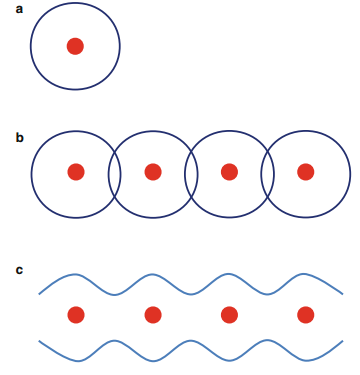
\includegraphics[width=6cm]{./images/tightbindPic.png} 
\caption{紧束缚模型原理。(a)假如只有一个原子则电子的波函数可以直接用单原子波函数表示。(b)但是在晶体中各个电子的单原子波函数会有一定的重叠。(c)这个重叠应该是比较小的,所以实际体系波函数可以用单原子波函数展开。\cite{topoText}}
\label{tightbindPic}
\end {figure} 
我们从简单的一维模型开始。图(\ref{tightbindPic}是一个简单的一维晶体,格点都是等间距排列。每一个格点可以表示材料中的一个原子。那么电子在这个体系里会处于什么状态呢?首先由于原子实的作用,电子会很喜欢待在一个格点上。但是量子力学的基本原理表明电子会有一定的概率跳到周边的格点上。这个跳跃的概率应该是比较小的。因为电子是费米子,如果旁边格点已经占据两个电子,则该格点的电子由于泡利原理的限制肯定无法进行跳跃。即使旁边格点仅有一个电子,电子和电子间的库伦排斥是相当强的,因此跳跃的概率也比较低。这样的话电子的波函数就可以被简单地写为该格点的原子波函数。

下面我们直观地考虑紧束缚模型是如何得到能带的。如果这个材料只有一个格点,那么它就
只有一个能级E。现在假设有两个间距很大的格点,则该系统的两个本征态——电子处于格点1
($\ket{\phi_1}$)和电子处于格点2($\ket{\phi_2}$),应该是简并的。这种情况下系
统还是只有一个能级E。假设这个间距被拉进,能级则会产生一些分裂$E =
E_{-1} + E_{1}$。一个比较直观的猜想就是这个分裂来源于两个波函数
$\ket{\phi_1}$和$\ket{\phi_2}$的交叠。如果以$\ket{\phi_1}$,$\ket{\phi_2}$ 为基底
的话,哈密顿量可以写成一个$2 \times 2$的矩阵。当两个格点距离非常远(波函数无交叠),哈密顿量是对角的
\begin{equation}
H =
\begin{bmatrix} 

    E & 0 \\

      0 & E

    \end{bmatrix}
    \end{equation}
而当距离较小时(波函数存在交叠),哈密顿量可以写为
\begin{equation}
H = 
\begin{bmatrix} 

    E & -t \\

      -t & E

    \end{bmatrix}
\end{equation}
其中t和波函数交叠有关,是导致能级分裂的非对角项。t可以表达为
\begin{equation}
  t = \hbar \omega \int{dx}|\phi_1^*(x) \phi_2(x)|^2
\end{equation}
这里的$\hbar$是普朗克常数,$\omega$是圆频率。因此$\hbar \omega$实质上赋予了交叠概率一个能量的量纲,使其能自然地成为哈密顿量的一部分。这个H对角化后的两个对角项分别为$E-t$和$E+t$,正是能级的分裂。
\section{一维简单紧束缚模型}
具有周期性边界条件的一维模型(图\ref{tightbindPic})的哈密顿量的非对角元可以被单独拆开来用产生湮灭算符来表示:
\begin{equation}
  \hat{H} = \sum_{ij} t_{ij} c_{i}^{\dagger} c_j
  \label{ham1dsimple}
\end{equation}
其中$i$和$j$为$0$到$N-1$的任一整数。其中N为模型的格点书。注意$\hat{H}$是厄米算子,因此要求$t_{ij} = t^*_{ji}$。以开边界且仅有最近邻相互作用的4格点长链为例,$t_{ij}$可以写为
\begin{equation}
\label{eq6}
t_{ij}=\left\{
\begin{aligned}
-t & , & |i - j| = 1, \\
0 & , & else.
\end{aligned}
\right.
\end{equation}
则H可以写为矩阵形式
\begin{equation}
H =
\begin{bmatrix} 

    0 & -t & 0 & 0 \\
    -t & 0 & -t & 0 \\
    0 & -t & 0 & -t \\
    0 & 0 & -t & 0 \\
  \end{bmatrix}
 \end{equation}
式子(\ref{ham1dsimple})可以通过对称性做一些简化。引入新变量n
\begin{equation}
  n = j - i
\end{equation}
代入(\ref{ham1dsimple})可得
\begin{equation}
  H = \sum_{n} \sum_i t_{i+n, i} c_{i+n}^\dagger c_i
\end{equation}
$t_{ij}$应该还具有平移对称性,即$t_{i+n, i}$不依赖于特定位置$i$的变量。因此$H$可以写为
\begin{equation}
  H = \sum_{n < N - i} t_n \sum_i c_{i+n}^\dagger c_i + h.c.
  \label{ham1dsimplified}
\end{equation}
接下来的步骤是对这个哈密顿量进行对角化处理。首先引入平移算子
\begin{equation}
  \hat{T} = \sum_i c_i c^\dagger_{i + 1}
\end{equation}
这个算子作用到格点$i + 1$上的波函数会得到格点$i $的波函数。而$\hat{T}^n$恰好为$H$的一项。因此(\ref{ham1dsimplified})又可以用平移算子表达
\begin{equation}
  H = - \sum_n t_n \hat{T}^n
\end{equation}
其中$t_n^* = t_{-n}$。显然这个哈密顿量平移算子对易,二者有相同的基。平移算子的基是算子的傅里叶变换
\begin{equation}
  C_k = \frac{1}{\sqrt{N}} \sum_j e^{ikj} c_j
\end{equation}
这里k的取值范围为$2 \pi m  / N$, $m$为整数. $\hat{T}$有本征值$e^{-ik}$。把这个代入哈密顿量可以得到一维晶格的本征值,也就是模型的能带
\begin{equation}
\epsilon(k) = - \sum_n t_n e^{-ikn}
\end{equation}

\section{原胞具有内部结构的情况}
实际上拓扑绝缘体所考虑的晶格模型的元胞都具有内部结构。下面以一维的,具有0号和1号两种类型晶格的一维点阵为例(图(\ref{tbInnerStruct}))来阐述这类模型的求解方法。

位于位置$i$的原子的算子可以被定义为$c_{i,a}$。若$a = 1$ 表示$1$号原子,$0$则为$0$号原子。一个通用的哈密顿量可以写成
\begin{equation}
H = \sum_{i, j} t_{ij}^{ab}c_{i,a}^{*}c_{j, b}
\label{ham1d}
\end{equation}
这里$t$的额外$a, b$指标取值分别也可以为$0, 1$, 可以表示不同原子间的相互作用。这个新的哈密顿量同样可以被平面波所对角化
\begin{equation}
  c_{k, a} = \frac{1}{\sqrt{N}} \sum_j e^{ikj} c_{j,a}
\end{equation}
它的傅里叶变换是
\begin{equation}
  c_{j, a} = \frac{1}{\sqrt{N}} \sum_j e^{-ikj} c_{k,a}
\end{equation}
代入(\ref{ham1d})式并利用模型的平移对称性化简可以得到
\begin{equation}
  H = - \sum_{n, k} t_n^{ab} e^{ikn} c_{k, a}c_{k, b}
\end{equation}
可以看出这个哈密顿量对于变量k来说是对角的,但是元胞的内部结构,即和a,b有关的量还不是对角。哈密顿量可以写成矩阵形式
\begin{equation}
        H = \begin{bmatrix}

        M^{ab}_{k_1}    &    &  & 0 \\
            &  M^{ab}_{k_2}  &  & \\

        &   & \ddots &  \\

        0  &  &   & M^{ab}_{k_N}


        \end{bmatrix}_{N \times N}
\end{equation}
其中$N$是原胞数目,$M^{ab}_k$是一个$m \times m$的小矩阵,$m$表示元胞内的原子数
在这个具体的模型里$m$为$2$,分别对应$0$号和$1$号原子.它的形式为
\begin{equation}
  M^{ab}_k = \sum_n t^{ab}_n e^{ikn}
\end{equation}
这个小矩阵实质上包含了原胞内部结构的信息。对角化矩阵$M^{ab}_k$可以得到模型的能带结构。一般来说原胞内有几种原子,就会有几个本征值,从而就能解出几个能带。
\begin {figure}[btp]
\centering 
\includegraphics[width=10cm]{./images/tbInnerStruct.jpg} 
\caption{原胞具有0,1两种原子的一维长链模型。任意两个格点之间都有相互作用。体系具有周期性边界}
\label{tbInnerStruct}
\end {figure} 
上述对一维模型的讨论也同样适用于二维晶格模型,只不过需要把最后结果的各个物理量换成二维矢量。
